\documentclass{article}
\usepackage[backend=biber]{biblatex}
\usepackage[german]{babel}
\usepackage{graphicx}
\usepackage{enumitem}
\usepackage{listings}
\usepackage{float}
\graphicspath{ {./img/} }

\setlength{\parindent}{0pt}

\bibliography{ByzantinischeFehler}

\title{Byzantinische Fehler}
\author{Matthias Reumann}
\date{\today}

\begin{document}

\maketitle

\newpage

\tableofcontents

\newpage

\iffalse
\section{Byzantinische Fehler}

\subsection{Definition}

Byzantinische Fehler treten in verteilten Systemen auf, 
wenn fehlerhafte Nachrichten von einem Knoten versendet werden, 
die von der Struktur und vom Inhalt nicht von fehlerfreien
unterscheidet werden können. \cite{esraberlin} 

\medskip 

Den Namen hat diese Fehlerklasse im Jahr 1982 von Lamport et. al. im 
Papier \textit{The Byzantine Generals Problem} erhalten.\cite{generals}
In diesem werden Byzantinische Fehler durch das abstrakte Beispiel 
der Byzantinischen Generäle beschrieben, dass im Abschnitt \ref{sec:generals} genauer erläutert wird.

\subsection{Problem}

Man stelle sich $n$ unabhängige Sensoren eines Notbremsassistenten vor, die miteinander kommunzieren.
Dabei werden nur Nachrichten \textit{STOP} oder \textit{OK} gesendet. Sobald einer der Sensoren, 
einen Wert misst, der unter eine Schranke $s$ fällt, teilt er dies den anderen $n-1$ Sensoren mit.

\medskip 

Hierbei ist die Aufgabe der Sensoren, eine gemeinsame Entscheidung zu fällen, ob gebremst werden soll. 
Oftmals wird dafür die absolute Mehrheit der Nachrichten verwendet. Diese Vorgehensweise funktioniert 
solange, bis ein Sensor fehlerhafte Informationen übermittelt, da keiner Sensoren die Fähigkeit besitzt die 
erhaltenen Informationen auf ihre Richtigkeit zu prüfen. Das könnte zu einer Fehlentscheidung führen 
und in Beispielen, wie dem Notbremsassistenten, fatale Folgen haben. 

\medskip 

Ein Beispiel eines solchen Byzantinischen Fehlers kann in Abbildung \ref{fig:example} gesehen werden. 

\begin{figure}[h]
    \centering
    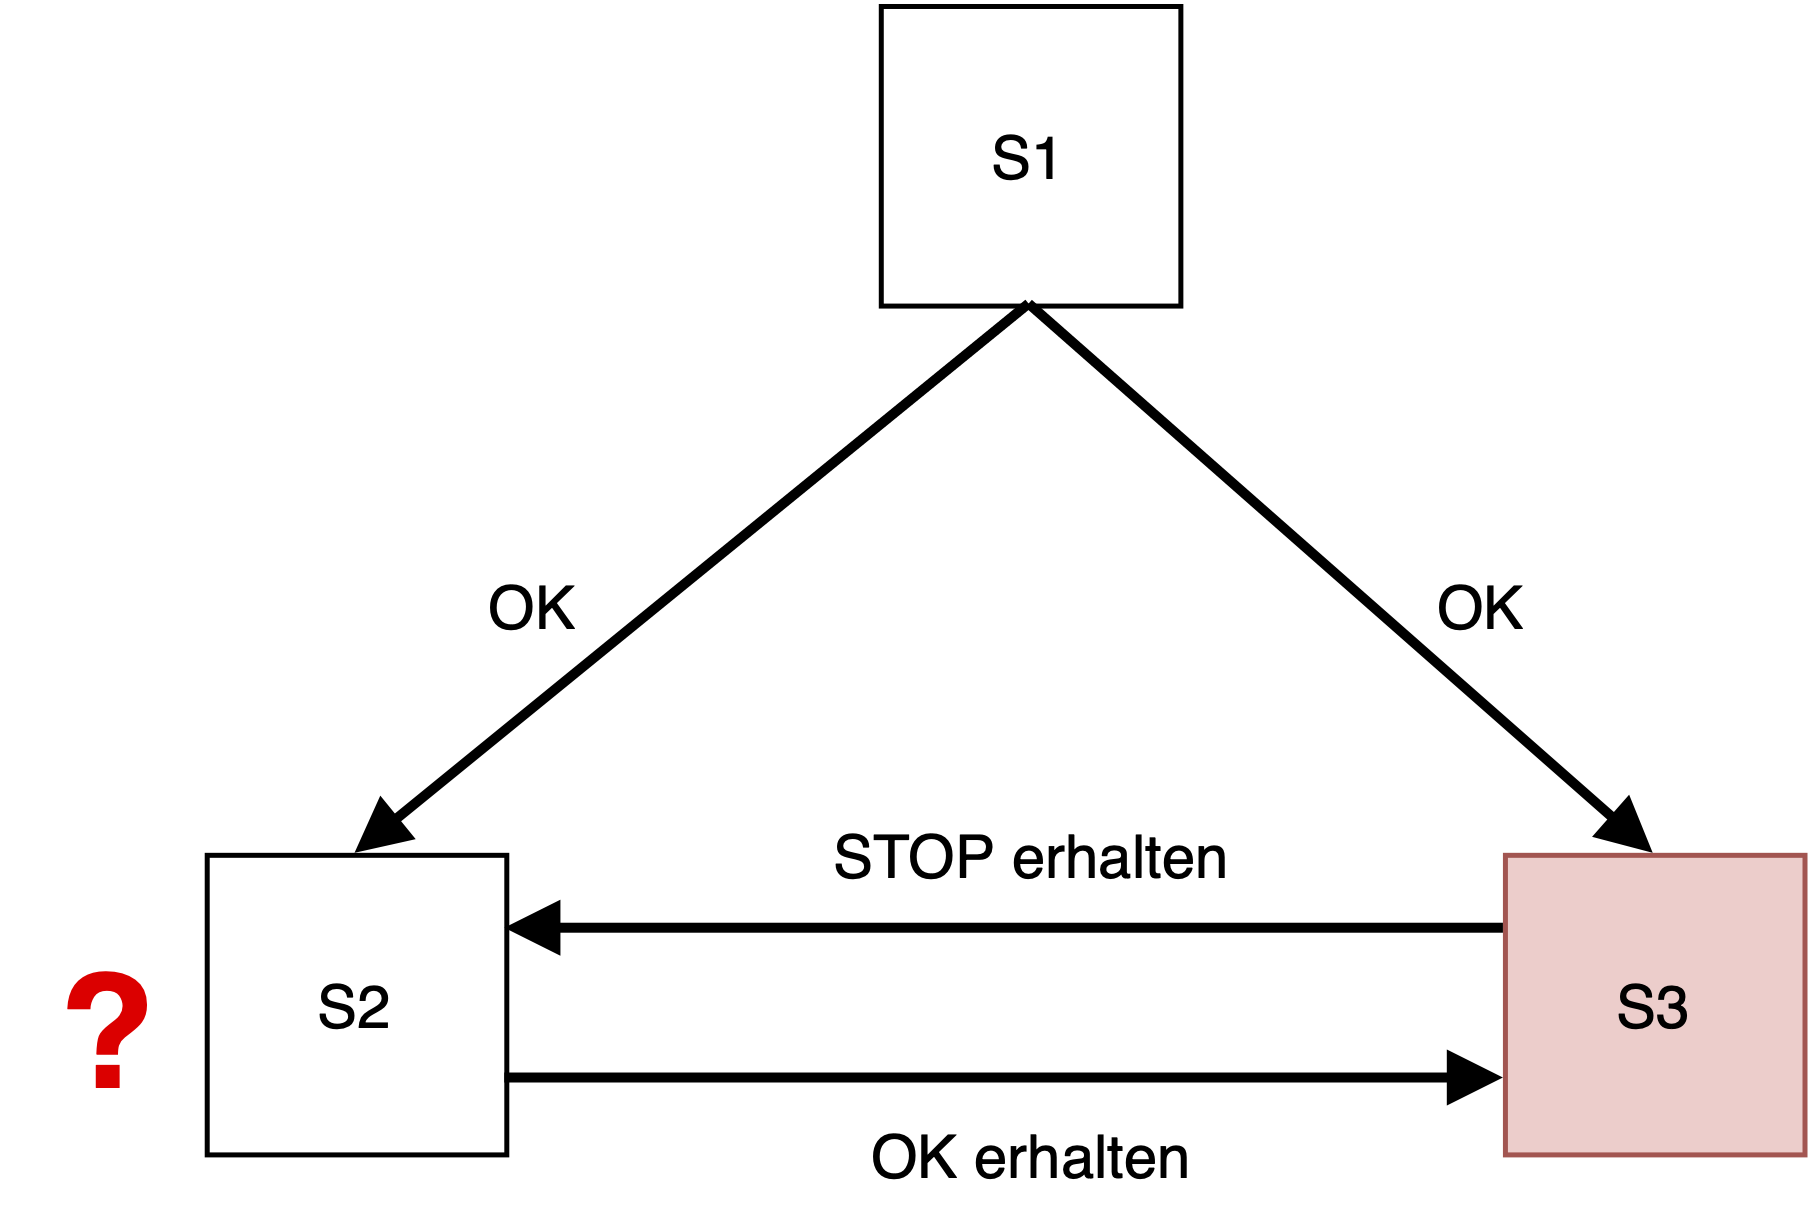
\includegraphics[width=0.7\textwidth]{byz-sensor-example.png}
    \caption{Sensornetzwerk mit fehlerhaftem Sensor 3. Für Sensor 2 ist es nicht möglich eine eindeutige Entscheidung zu treffen.}
    \label{fig:example}
\end{figure}

\medskip 

\fi

\section{Problem der byzantinischen Generäle}
\label{sec:generals}

Mehrere Truppen mit jeweils einem General umzingeln eine feindliche Stadt und 
kommunizieren direkt über Boten miteinander. 
Jeder der Generäle beobachtet den Feind und schlussendlich müssen die Generäle 
eine gemeinsame Entscheidung treffen. Jedoch kann es unter den Generälen Verräter geben,
deren Ziel es ist eine gemeinsame Entscheidung der loyalen Generäle zu unterbinden. 

\medskip 

Die Generäle müssen einen Algorithmus finden der garantiert, dass

\begin{enumerate}[label=(\alph*)]
\item Alle loyalen Generäle die gleiche Entscheidung treffen 
\item Eine geringe Anzahl an Verrätern die loyalen Generäle nicht zu einer Fehlentscheidung führt
\end{enumerate}

Eine Entscheidung unter den Generälen wird gefällt 
indem jeder General den Feind beobachtet und seine
Informationen an die anderen Generäle weitergibt. \textit{v(i)} ist die 
Nachricht gesendet vom $i$.ten General. Jeder General erhält die Nachrichten 
\textit{v(1)} bis \textit{v(n)}, wobei $n$ die Anzahl der Generäle darstellt. 
Die finale Entscheidung wird durch die absolute Mehrheit der Werte dieser Nachrichten
bestimmt. Allerdings könnte es sein, dass loyale Generäle unterschiedliche \textit{v(i)}
erhalten, da ein Verräter unterschiedliche Werte zu unterschiedlichen Generälen sendet, 
was widerum Punkt A widerspricht. 

\medskip 

Deshalb müssen sogennante \textit{interactive consistency}-Bedingungen gelten.
Ein führender General, auch Commander gennant, sendet einen Befehl an seine $n - 1$ Leutnant 
Generäle so, dass:

\smallskip 

\begin{tabular}{l l}
IC1 & Alle loyalen Leutnants den gleichen Befehl ausführen \\
IC2 & Wenn der Commander loyal ist, dann befolgt jeder loyale Leutnant seinen Befehl
\end{tabular}

\subsection{Beispiel mit drei Generälen}
In diesem Abschnitt wird ein Bespiel beschrieben in dem drei Generäle miteinander kommunzieren. 
Wichtig dabei ist, dass niemand der loyalen Generäle weiß wer der Verräter ist. 

\medskip

In Abbildung \ref{fig:general1} ist Leutnant 2 (L2) der Verräter. Der loyale Commander
sendet den Befehl \textit{ANGRIFF} an beide Leutnants L1 und L2. Zur Verifizierung sendet L2 L1 die Nachricht,
er habe den Befehl \textit{RÜCKZUG} erhalten. Um die IC2 zu erfüllen, muss L1 jedoch
den Befehl des Commanders ausführen. 

\begin{figure}[H]
    \centering
    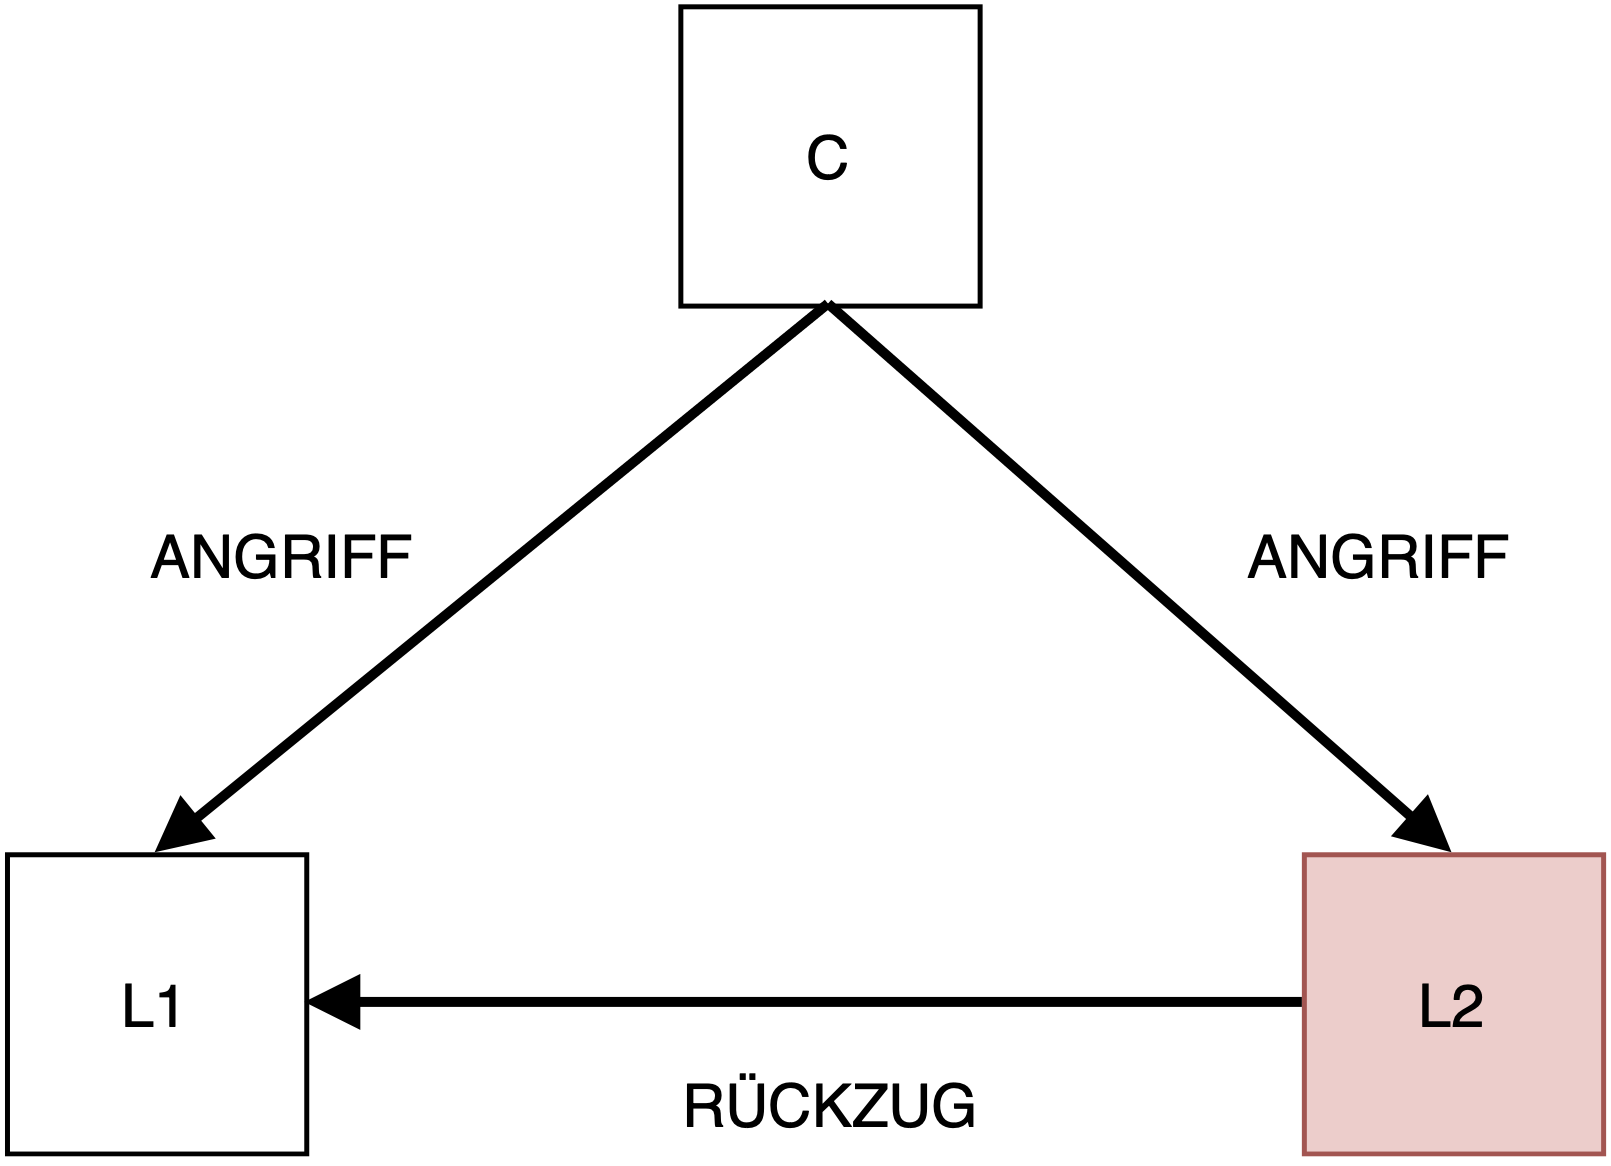
\includegraphics[width=0.7\textwidth]{general1.png}
    \caption{L2 ist der Verräter. L1 muss den Befehl des Commanders auführen um die IC2 einzuhalten.}
    \label{fig:general1}
\end{figure}

Im nächsten Szenario (Abbildung \ref{fig:general2}) ist der Commander der Verräter. Dieser sendet unterschiedliche 
Befehle an L1 und L2. Für L1 ist es die exakt selbe Situation 
wie in Abbildung \ref{fig:general1}: Um die IC2 zu erfüllen muss er den Befehl \textit{ANGRIFF} ausführen. 

\begin{figure}[H]
    \centering
    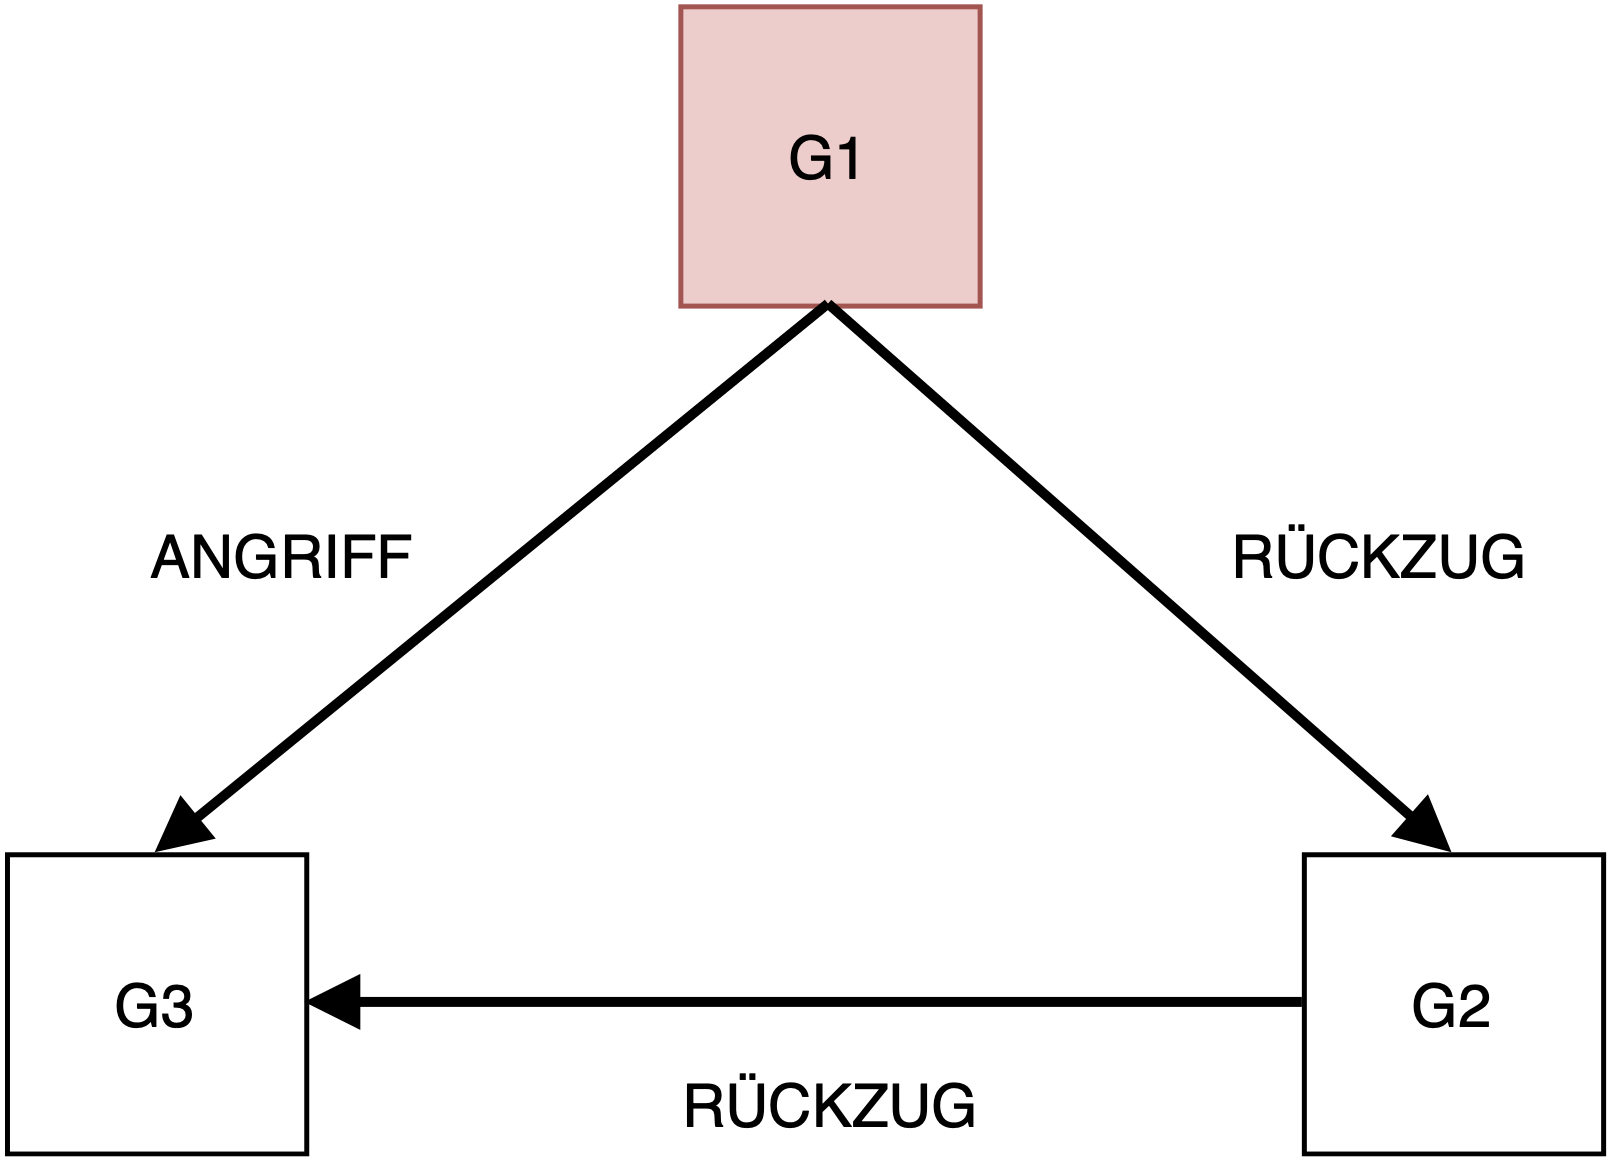
\includegraphics[width=0.7\textwidth]{general2.png}
    \caption{Der Commander ist der Verräter. Für L1 ist es die selbe Situtation wie in Abbildung \ref{fig:general1}.}
    \label{fig:general2}
\end{figure}

Hierbei liegt aber das Problem. Die gleiche Argumentation muss demnach für L2
verwendet werden, der den Befehl \textit{RÜCKZUG} ausführt. Dies widerspricht jedoch 
IC1. Es existiert daher keine Lösung für drei Generäle mit einem Verräter. 
Um einen byzantinischen Fehler zu erkennen muss daher folgende Eigenschaft gelten: $n \geq 3m + 1$, 
wobei n die Anzahl der Generäle und m die Anzahl der Verräter in diesem System ist.

\subsection{Lösung}

Eine mögliche Lösung dieses Problems bietet der Oral-Message-Algorithmus, kurz OM-Algorithmus. Der
Algorithmus funkioniert für Systeme die die Eigenschaft $n \geq 3m + 1$ erfüllen. Außerdem werden 
folgende Annahmen getroffen: \\

\begin{itemize}
    \item Jede Nachricht wird korrekt empfangen 
    \item Der Empfänger kann sicherstellen von wem die Nachricht versendet wurde 
    \item Fehlende Nachrichten können erkannt werden
\end{itemize}

Der Algorithmus funktioniert nur wenn ein General mit jedem anderen General 
direkt miteinander kommunzieren kann. Ein Verräter-Commander könnte auch 
keinen Befehl an seine Leutnants senden, daher ist der Standardbefehl in diesem 
Fall \textit{RÜCKZUG}.

\begin{lstlisting}[caption=Algorithmus OM(0)]
1) Commander sendet seinen Wert v0 an alle Leutnants
2) Jeder Leutnant verwendet den Wert v0 oder 
  falls dieser nicht vorhanden ist den Standardbefehl
\end{lstlisting}

\medskip

\begin{lstlisting}[caption=Algorithmus OM(m) m > 0]
1) Commander sendet seinen Wert v0 an alle Leutnants
2) Für jedes i gilt:
    vi := Wert den General i vom Commander erhalten hat 
    (oder Standardbefehl)
    General i agiert wie der Commander im OM(m-1) um seinen 
    Wert vi den anderen n-2 Generälen zu senden

3) Für jedes i mit j != i gilt:
    vj := Wert den General i von General j in Schritt 2 erhalten hat
    General i benutzt die Funktion majority(v1, vn-1)
\end{lstlisting}

Die Funktion \textit{majority} ermittelt die absolute Mehrheit. 
Es muss nicht immer die absolute Mehrheit als Entscheidungsfunktion verwendet werden.


\iffalse

\subsection{Kritik}

Der OM-Algorithmus ist sehr aufwendig. Er ist praktisch nicht für große $n$ und $m$ einsetzbar.  

\subsection{Beispiel}

\newpage 

\printbibliography

\fi


\end{document}